
% Chapter 

\chapter{Co-evolution at the meso-scale}{Co-évolution à l'Echelle Mesoscopique}

\label{ch:mesocoevolution} 

%----------------------------------------------------------------------------------------


% - tests with rbd, extentded rbd with different heuristics ; simple coupling of density with nw ?











%--------------------------------------

\newpage

\section[Co-evolution at the meso scale][Co-évolution à l'échelle mesoscopique]{Co-evolution of forms: interactions and morphogenesis at the meso scale}{Co-evolution des formes : interactions et morphogenèse à l'échelle mesoscopique}












%--------------------------------------

% Section : benchmarking of network growth models

\newpage

\section[Network Growth Models]{Network Growth Models : Explicative power for various approaches}{Modèles de Croissance de Réseau}

\subsection{Benchmarking Network growth heuristics}{Comparer les heuristiques de croissance de réseau}


\bpar{
Considering Network Growth in itself, many heuristics are available to generate a network under some constraints. As already developed, from economic network growth approach to local optimization heuristics, geographical mechanisms or biological network growth, each has its advantages and particularities. We plan to compare these varied methods against real network indicators values for the european road network. We present in Fig.~\ref{fig:slimemould} a preliminary work done in~\cite{raimbault2015labex} to explore implementation of the biological network growth models. Also the implementation of local optimization models was explored, typically the one described in the methodology section on reproducibility. 
}{
\comment{(Florent) cela doit remonter avant ton modèle : on est encore dans l'état de l'art}
Pour la croissance du réseau en tant que tel, de nombreuses heuristiques existent pour générer un réseaux sous certaines contraintes. Comme déjà développé précédemment, des modèles économiques de croissance de réseau au heuristiques d'optimisation locale, aux mécanismes géographiques ou à la croissance de réseau biologique, chacun a ses avantages et particularités propres. Un travail futur aura pour but de comparer ces diverses méthodes contres les valeurs réelles des indicateurs pour le réseau de routes européen. La Fig.~\ref{fig:slimemould} présente un travail préliminaire présenté dans~\cite{raimbault2015labex} qui explore des applications des modèles de croissance de réseau biologique. D'autre part, comme présenté dans la section sur la reproductibilité, des modèles d'optimisation locale ont également été testés.
}


%%%%%%%%%%%%%%%%%%%%%%
\begin{figure}
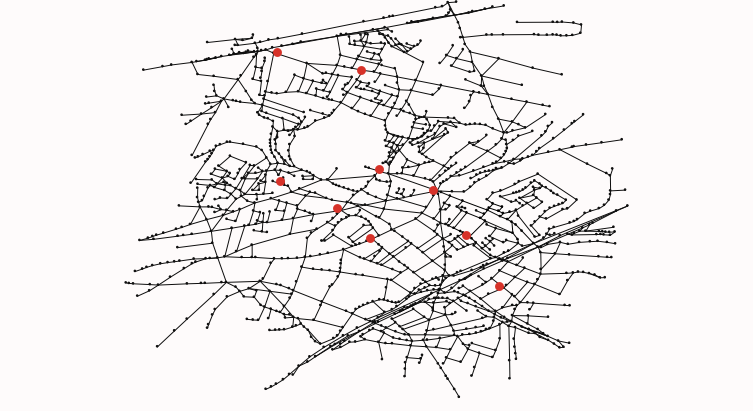
\includegraphics[width=0.45\textwidth]{Figures/NetworkGrowth/tick1}
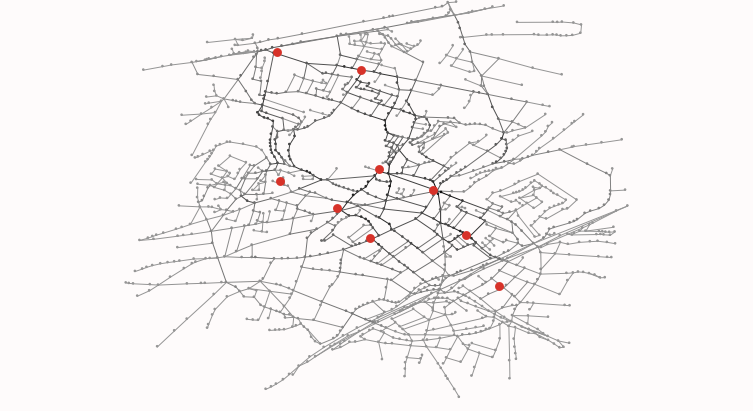
\includegraphics[width=0.45\textwidth]{Figures/NetworkGrowth/tick20}\\
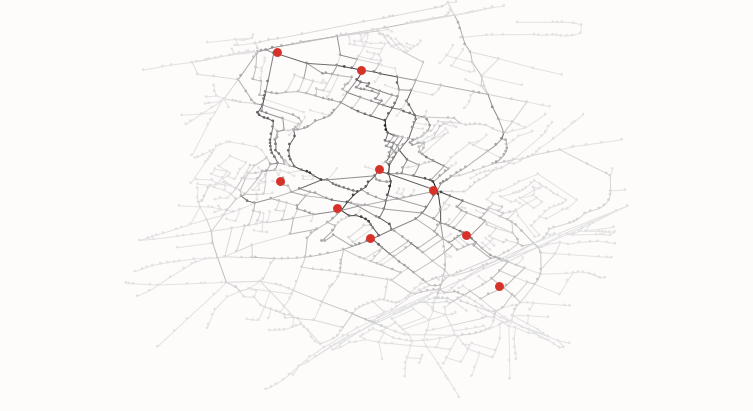
\includegraphics[width=0.45\textwidth]{Figures/NetworkGrowth/tick50}
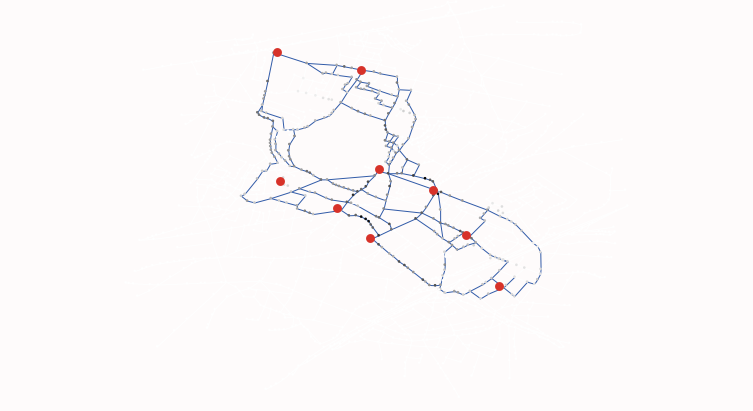
\includegraphics[width=0.45\textwidth]{Figures/NetworkGrowth/reseauFinal}
\caption[Biological Network Growth][Croissance de réseau biologique]{Example of the application of the slime mould network generation model to the computation of an optimal public transportation network design.}{\comment{(Florent) source ?}}
\label{fig:slimemould}
\end{figure}
%%%%%%%%%%%%%%%%%%%%%%%



\todo{pour pouvoir comparer ``toutes choses égales par ailleurs'' les différentes heuristiques de génération de réseau, il est nécessaire des les explorer à densité fixée $\rightarrow$ cf thèse Mimeur et Morphogenesis ?}





%\subsection{Towards simple models of network morphogenesis}{Vers des modèles simples de morphogenèse de réseau}

%\todo{this part may be skipped or put in targeted potential developments if nothing is done before Nov. 2017}

%An interdisciplinary project that was just launched with a Physicist \noun{Lagesse}, an Architect \noun{Hachi} and a Computer Scientist \noun{Dugue} aims at finding consistent models of urban street network morphogenesis, regarding urban design particularities, geographical rules and complex network indicators feedbacks. Models of network morphogenesis were already discuss here and the aim of this project is to gain insight from the interdisciplinary vision to explore the potentiality of such models. In the frame of our thesis, it is logically situated within the morphogenesis theoretical part and network growth modeling heuristics.





